\section{Experiments}\label{sec:exp}

The previous sections prove the static-\cpi{} invariant and derive two ways to compute the same fixed point: the direct \spin{} solver and the practical \spinStar{} realization.
%
The comparison with \cbnd{} is therefore a cost comparison, while exactness comes from the invariants and fixed-point equivalence proved earlier.
%
They ask whether the static pipeline changes the cost profile enough to matter.
%
\textbf{RQ1} measures end-to-end time and peak memory for \textbf{\spinStar{}}, the practical static-\cpi{} pipeline.
%
\textbf{RQ2} separates construction from peeling, because counter-only peeling shifts rather than removes all cost.
%
\textbf{RQ3} asks whether the static construction contract gives useful parallelism.
%
\textbf{RQ4} measures \spin{} as the direct fixed-point baseline.
%
\textbf{RQ5} probes dense synthetic graphs where clique counts grow quickly.

\stitle{Hardware and software.}
All experiments run on a dual-socket Intel Xeon Gold \(6248R\) machine with \(24\) cores and \(503\) GB DDR4 memory.
%
The operating system is Ubuntu \(22.04\).
%
The code is compiled with Clang \(18.1\) using \texttt{-O3 -march=native}.
%
It is linked against TBB \(2021.10\), Boost \(1.83\), and \texttt{robin\_hood::unordered\_flat\_map}.
%
Single-threaded measurements use one core.
%
Parallel-construction measurements use the thread counts reported in Table~\ref{tab:par}.
%
Wall-clock and resident-set measurements are averaged or summarized over repeated runs as stated in each experiment.

\stitle{Datasets.}
Table~\ref{tab:datasets} lists the benchmark graphs.
%
The set covers collaboration, e-commerce, social, and web graphs.
%
The largest graph is \texttt{com-orkut} with \(117\)M edges.
%
The benchmark sweep covers \(762\) \((graph,s)\) configurations across the ten graphs (Table~\ref{tab:datasets}); \(307\) of these are matched cells where both \spinStar{} and \cbnd{} complete successfully, and the headline speedup numbers are reported over the matched subset.

\begin{table}[t]
\centering
\caption{Datasets used in Section~\ref{sec:exp}. The last column gives the number of \((graph,s)\) configurations included in the benchmark sweep.}
\label{tab:datasets}
\small
\begin{tabular}{lrrr}
\toprule
Graph & \(|V|\) & \(|E|\) & \# \((g,s)\) \\
\midrule
\texttt{com-amazon}~\cite{communityFinder}      & \(334{,}863\)    & \(925{,}872\)       & \(29\) \\
\texttt{com-dblp}~\cite{communityFinder}        & \(317{,}080\)    & \(1{,}049{,}866\)   & \(109\) \\
\texttt{twitter}~\cite{communityFinder}         & \(\phantom{0,0}81{,}306\) & \(1{,}342{,}296\) & \(29\) \\
\texttt{web-Stanford}~\cite{communityFinder}    & \(281{,}903\)    & \(1{,}992{,}636\)   & \(60\) \\
\texttt{com-youtube}~\cite{communityFinder}     & \(1{,}134{,}890\) & \(2{,}987{,}624\)   & \(16\) \\
\texttt{web-Google}~\cite{communityFinder}      & \(875{,}713\)    & \(4{,}322{,}051\)   & \(39\) \\
\texttt{wiki-Talk}~\cite{communityFinder}       & \(2{,}394{,}385\) & \(4{,}659{,}565\)   & \(24\) \\
\texttt{web-it-2004}~\cite{communityFinder}     & \(509{,}338\)    & \(7{,}178{,}413\)   & \(429\) \\
\texttt{soc-pokec}~\cite{communityFinder}       & \(1{,}632{,}803\) & \(22{,}301{,}964\)  & \(24\) \\
\texttt{com-orkut}~\cite{communityFinder}       & \(3{,}072{,}441\) & \(117{,}185{,}083\) & \(3\) \\
\midrule
\textbf{Total} & & & \(762\) \\
\bottomrule
\end{tabular}
\end{table}

\stitle{Algorithms and methodology.}
\textbf{\cbnd{}} is the mutable-\cpi{} implementation of general \((r,s)\)-nucleus decomposition~\cite{NuclearCD}, restricted to \(r=1\) for this comparison.
%
It maintains the \cpi{} as mutable residual state: each peel step deletes the popped vertex from every path that references it, rewrites the affected path records, and updates a hash-indexed reverse map so the next pop can locate its incident paths.
%
The dominant per-pop cost is therefore the residual-index rewrite plus the hash-set rebuild that reflects the deletion; this work is intrinsic to the mutable design and is what \spinStar{} avoids by leaving the \cpi{} unchanged.
%
\textbf{\spinStar{}} is the practical static-\cpi{} pipeline.
%
It constructs the static index, stores flat incidence arrays, and computes core values by incremental path-counter updates.
%
\spin{} is evaluated separately because it is the direct fixed-point formulation rather than the practical implementation.
%
All three solvers consume the same input edge list and run on the same hardware.
%
The comparison isolates the cost of \cpi{} mutability against static-state peeling, not differences in input processing or execution environment.

For every matched \((graph,s)\) pair, we run \cbnd{} and \spinStar{} on the same input.
%
We record end-to-end wall-clock time and peak resident-set memory from \texttt{getrusage}'s \texttt{ru\_maxrss}.
%
End-to-end time includes graph loading, degeneracy ordering, \cpi{} construction, peeling, and output emission.
%
The exactness claim comes from Theorem~\ref{thm:vertex-removal}, Lemma~\ref{lem:hindex-fixed-point}, and Lemma~\ref{lem:equivalence}.

\stitle{RQ1: end-to-end time and memory.}
The benchmark has \(307\) matched cells where both \spinStar{} and \cbnd{} complete.
%
Across the ten graphs, \spinStar{} achieves a peel-time speedup over \cbnd{} of geometric-mean \(13.50\times\) and maximum \(44.76\times\).
%
The end-to-end wall-clock speedup is smaller (gmean \(1.10\times\)) because the shared SDCT construction phase dominates total wall time once peeling is cheap; this is the bottleneck shift that motivates \paraBuild{} in Section~\ref{sec:parabuild}.
%
The peak-RSS ratio (\cbnd{} over \spinStar{}) has geometric mean \(1.55\times\) and maximum \(3.92\times\).
%
Figure~\ref{fig:exp-time} and Figure~\ref{fig:exp-mem} show where these gains occur.

\begin{figure*}[t]
\centering
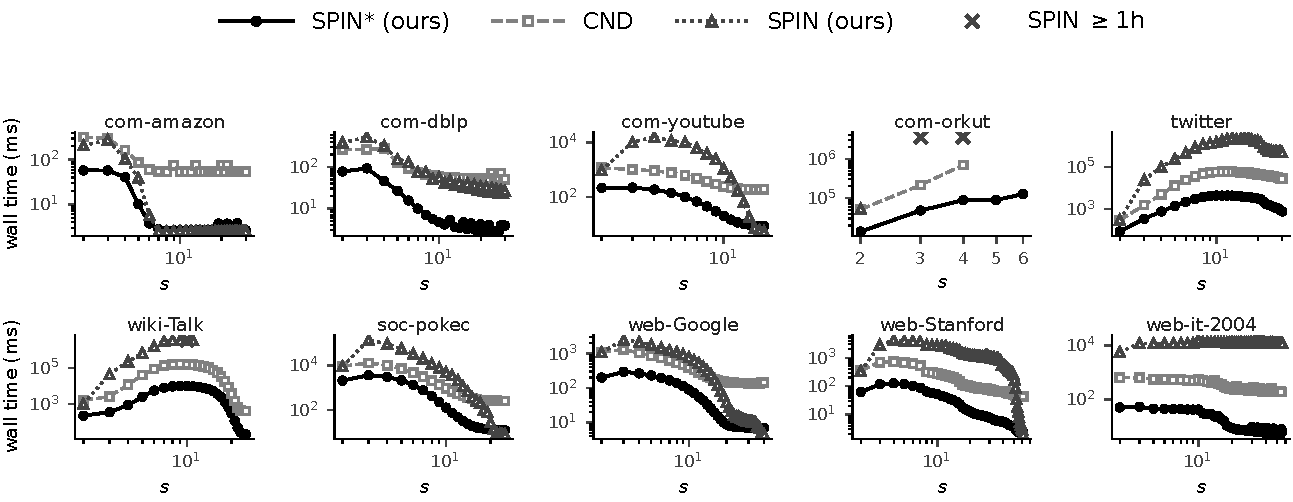
\includegraphics[width=\linewidth]{figures/fig_exp_time.pdf}
\caption{End-to-end wall-clock time as a function of \(s\) in the ten-graph comparison.
%
Solid black is \spinStar{}, the incremental realization; dashed gray is the mutable-\cpi{} reference baseline \cbnd{}; dotted dark gray is \spin{}, the direct iteration.
%
Crosses (\(\times\)) mark cells where \spin{} exceeded the \(1\)h wall-clock cap.
%
\spinStar{} is consistently the fastest; \cbnd{} pays residual-index maintenance cost; \spin{} pays for repeated full-graph passes and times out on the harder graphs.}
\Description{A grid of log-scale runtime plots over parameter s, with one subplot per benchmark graph.}
\label{fig:exp-time}
\end{figure*}

\begin{figure*}[t]
\centering
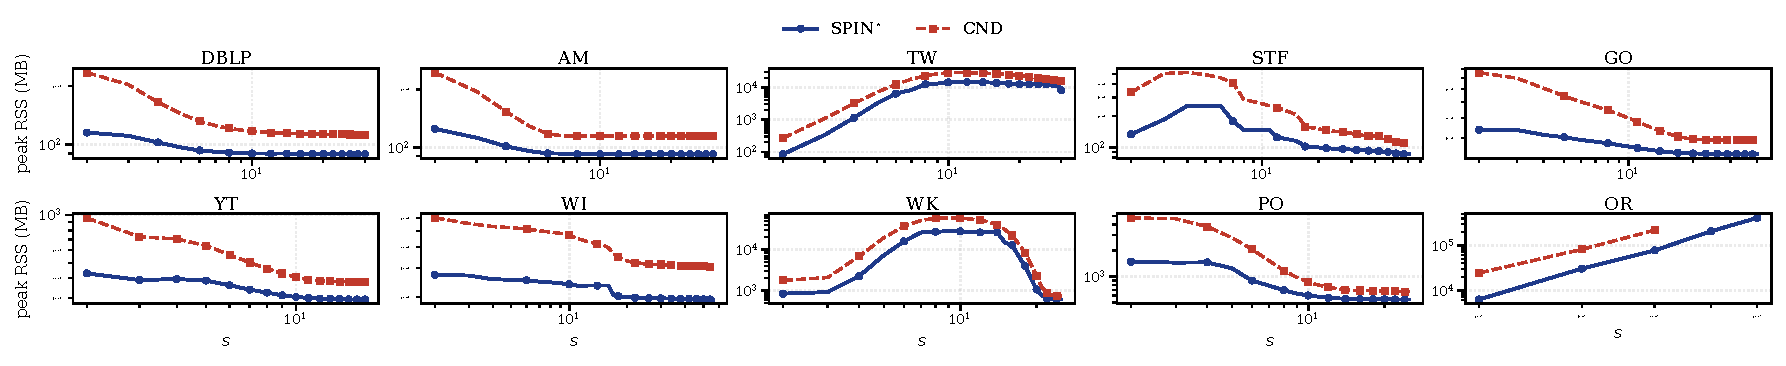
\includegraphics[width=\linewidth]{figures/fig_exp_mem.pdf}
\caption{Peak resident-set memory in the ten-graph comparison.
%
Solid black is \spinStar{}; dashed gray is \cbnd{}; dotted dark gray is \spin{}.
%
The static incidence layout reduces peak RSS when mutable residual path sets dominate memory.
%
\spin{} now reads paths from the same flat dual CSR as \spinStar{}, so its curve tracks \spinStar{}'s closely instead of carrying the legacy vector-of-vectors overhead.}
\Description{A grid of log-scale peak-memory plots over parameter s, with one subplot per benchmark graph.}
\label{fig:exp-mem}
\end{figure*}

Figure~\ref{fig:exp-endtoend} focuses on the three graphs used in the detailed phase study.
%
It contains \(130\) matched configurations.
%
On those cells, the geometric-mean peel-time speedup of \spinStar{} over \cbnd{} is \(14.62\times\).
%
The maximum peel-time speedup is \(44.76\times\).
%
Peak-RSS ratio has \(1.58\times\) geometric mean and \(2.75\times\) maximum.

\begin{figure*}[t]
\centering
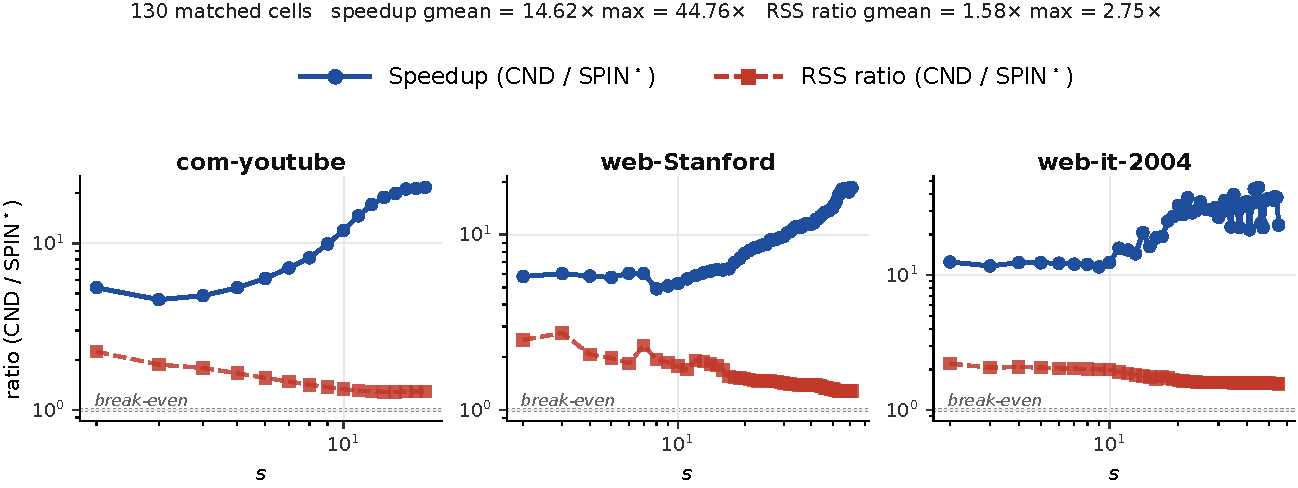
\includegraphics[width=\linewidth]{figures/fig_exp_endtoend.pdf}
\caption{Speedup and peak-RSS ratio on \texttt{com-youtube}, \texttt{web-Stanford}, and \texttt{web-it-2004}.
%
The curves show \cbnd{} divided by \spinStar{} on matched successful configurations.
%
Values above \(1\) mean \spinStar{} is faster or uses less memory.}
\Description{Three-panel plot comparing speedup and memory ratio between \spinStar{} and the mutable baseline on the matched subset.}
\label{fig:exp-endtoend}
\end{figure*}

The memory improvement is explained by the incidence-level budget in Table~\ref{tab:mem}.
%
The mutable baseline stores path hash sets and reverse hash maps.
%
\spinStar{} stores flat path-to-vertex and vertex-to-path arrays plus path counters.
%
The analytical per-incidence gap is larger than the observed RSS gap because graph adjacency, allocator overhead, and per-vertex structures do not scale with \(\Sig\).

\begin{table}[t]
\centering
\caption{Memory budget per vertex--path incidence at \(\Sig\gg n\).
%
Baseline numbers are from the mutable-\cpi{} implementation~\cite{NuclearCD}.
%
\spinStar{} numbers are sizeof-based accounting for the static layout.}
\label{tab:mem}
\small
\begin{tabular}{lrr}
\toprule
\textbf{Component} & \textbf{Baseline} & \textbf{\spinStar{}} \\
\midrule
BK recursion tree \(\mathsf{T}\) & \(8\Sig\) & \(0\) \\
Path-to-vertex storage \((V_h,V_p)\) & \(0\) & \(4\Sig\) \\
Per-path vertex set \(\mathsf{H}_P\) & \(32\Sig\) & --- \\
Reverse vertex-to-path map & \(48\Sig\) & --- \\
Vertex-to-path incidence & --- & \(4\Sig\) \\
Support array & \(4n\) & \(4n\) \\
Heap / bucket array & \(24n\) & \(16n+8\kmax\) \\
\midrule
\textbf{Dominant total} & \(\approx 88\Sig\) & \(\approx 10\Sig\) \\
\bottomrule
\end{tabular}
\end{table}

\stitle{RQ2: where does the time go?}
The static invariant makes peeling cheap, so the next question is whether construction becomes the dominant cost.
%
The phase study uses \texttt{com-youtube}, \texttt{web-Stanford}, and \texttt{web-it-2004}.
%
It reports median times over three runs.
%
Table~\ref{tab:bd-time} reports representative phase medians.
%
Table~\ref{tab:bd-mem} reports the corresponding memory medians.

\begin{table}[t]
\centering
\caption{Representative per-phase wall-clock time in ms, median over three runs.}
\label{tab:bd-time}
\scriptsize
\begin{tabular}{llrrrrrr}
\toprule
\multirow{2}{*}{Graph} & \multirow{2}{*}{\(s\)} & \multicolumn{3}{c}{\spinStar{}} & \multicolumn{3}{c}{\cbnd{}} \\
\cmidrule(l){3-5}\cmidrule(l){6-8}
& & load & build & peel & load & build & peel \\
\midrule
\texttt{com-youtube}  & 3  & 2081 & 3863 & 440.1 & 1812 & 3982 & 789.7 \\
\texttt{com-youtube}  & 5  & 2028 & 3730 & 273.5 & 1732 & 3795 & 581.6 \\
\texttt{com-youtube}  & 8  & 1967 & 2991 & 86.3  & 1638 & 3053 & 270.2 \\
\texttt{com-youtube}  & 12 & 1689 & 2701 & 13.0  & 1640 & 2649 & 148.5 \\
\texttt{com-youtube}  & 16 & 1640 & 2458 & 8.2   & 1964 & 2488 & 131.8 \\
\midrule
\texttt{web-Stanford} & 3  & 1251 & 6602 & 381.6 & 1250 & 6548 & 521.5 \\
\texttt{web-Stanford} & 10 & 975  & 5840 & 130.4 & 1225 & 5961 & 210.1 \\
\texttt{web-Stanford} & 20 & 999  & 5482 & 28.9  & 1228 & 5591 & 77.8 \\
\texttt{web-Stanford} & 40 & 1224 & 5087 & 9.6   & 1034 & 5007 & 49.6 \\
\texttt{web-Stanford} & 60 & 1224 & 4900 & 1.4   & 1224 & 4907 & 31.3 \\
\midrule
\texttt{web-it-2004}  & 3   & 3389 & 124074 & 351.0 & 3378 & 125347 & 465.9 \\
\texttt{web-it-2004}  & 30  & 3372 & 122558 & 63.9  & 3037 & 122689 & 173.7 \\
\texttt{web-it-2004}  & 100 & 3407 & 121891 & 40.1  & 3377 & 121372 & 135.9 \\
\texttt{web-it-2004}  & 200 & 3416 & 113825 & 26.1  & 3406 & 107516 & 108.5 \\
\texttt{web-it-2004}  & 400 & 3409 & 7850   & 4.6   & 3368 & 7847   & 62.7 \\
\bottomrule
\end{tabular}
\end{table}

\begin{table}[t]
\centering
\caption{Representative peak resident-set memory in MB, median over three runs.}
\label{tab:bd-mem}
\small
\begin{tabular}{llrrr}
\toprule
Graph & \(s\) & \spinStar{} & \cbnd{} & Ratio \\
\midrule
\texttt{com-youtube}  & 3  & 381 & 729 & \(1.91\times\) \\
\texttt{com-youtube}  & 5  & 315 & 642 & \(2.04\times\) \\
\texttt{com-youtube}  & 8  & 187 & 460 & \(2.45\times\) \\
\texttt{com-youtube}  & 12 & 119 & 385 & \(3.25\times\) \\
\texttt{com-youtube}  & 16 & 114 & 380 & \(3.33\times\) \\
\midrule
\texttt{web-Stanford} & 10 & 176 & 261 & \(1.48\times\) \\
\texttt{web-Stanford} & 40 & 70  & 129 & \(1.85\times\) \\
\texttt{web-Stanford} & 60 & 53  & 111 & \(2.09\times\) \\
\midrule
\texttt{web-it-2004}  & 3   & 425 & 556 & \(1.31\times\) \\
\texttt{web-it-2004}  & 100 & 207 & 296 & \(1.43\times\) \\
\texttt{web-it-2004}  & 400 & 139 & 227 & \(1.63\times\) \\
\bottomrule
\end{tabular}
\end{table}

The phase data supports the bottleneck-shift story.
%
Peeling falls to tens or hundreds of milliseconds on many cells.
%
Construction then becomes a major remaining cost, especially on the web graphs.
%
This is why \paraBuild{} is part of the algorithmic pipeline rather than a detached engineering detail.

\stitle{RQ3: does static construction parallelize?}
\paraBuild{} exposes seed-level parallelism because each seed can stream its emitted paths into thread-local storage.
%
Table~\ref{tab:par} reports build time as the thread count grows from \(1\) to \(24\).
%
Each cell is the median of three runs.
%
The table shows strong scaling on large web and social graphs and weaker scaling on smaller overhead-dominated cases.

\begin{table}[t]
\centering
\caption{\paraBuild{} build time in ms, median over three runs.
%
Speedup is \(T=1\) time divided by \(T=24\) time.}
\label{tab:par}
\tiny
\setlength{\tabcolsep}{2pt}
\begin{tabular}{@{}llrrrrrrr@{}}
\toprule
Graph & \(s\) & \(T=1\) & \(T=2\) & \(T=4\) & \(T=8\) & \(T=16\) & \(T=24\) & sp. \\
\midrule
\texttt{com-dblp}      & 3   & 205   & 131   & 84    & 61    & 56   & 58   & \(3.5\times\) \\
\texttt{com-dblp}      & 15  & 182   & 115   & 73    & 51    & 43   & 45   & \(4.0\times\) \\
\texttt{dblp-core30}   & 3   & 47    & 36    & 28    & 25    & 22   & 22   & \(2.1\times\) \\
\texttt{com-youtube}   & 3   & 2644  & 1516  & 833   & 465   & 275  & 214  & \(12.4\times\) \\
\texttt{com-youtube}   & 16  & 2418  & 1367  & 744   & 399   & 224  & 168  & \(14.4\times\) \\
\texttt{web-Stanford}  & 3   & 5357  & 2776  & 1538  & 834   & 458  & 331  & \(16.2\times\) \\
\texttt{web-Stanford}  & 60  & 5196  & 2697  & 1483  & 793   & 422  & 297  & \(17.5\times\) \\
\texttt{web-it-2004}   & 3   & 92312 & 49798 & 26304 & 13048 & 5789 & 3946 & \(23.4\times\) \\
\texttt{web-it-2004}   & 400 & 83795 & 45977 & 24673 & 10935 & 5863 & 3930 & \(21.3\times\) \\
\bottomrule
\end{tabular}
\end{table}

The correct interpretation is not that construction is perfectly parallel.
%
It is that static output removes hot-path residual-index mutation from the seed walks.
%
This lets the expensive enumeration work scale until memory bandwidth and scheduling overhead become visible.

\stitle{\texorpdfstring{RQ4: how much does \spinStar{} optimize over \spin{}?}{RQ4: how much does SPIN* optimize over SPIN?}}
\spin{} is the literal single-thread solver for the same equations that \spinStar{} realizes by deletion events.
%
The two algorithms compute the same core values (Lemma~\ref{lem:equivalence}), so the comparison isolates the effect of replacing repeated full-graph passes with incremental updates.
%
Both implementations read paths from the same flat dual CSR; the SPIN reference therefore reflects the algorithmic cost of repeated full-pass fixed-point iteration, not data-structure overhead.
%
Figure~\ref{fig:spin-vs-spinstar} pairs \spin{} and \spinStar{} on the \(291\) matched \((graph,s)\) cells.
%
The geometric-mean peel-time speedup is \(36.2\times\) over the full set; the hardest \(20\) cells (those shown) reach gmean \(2{,}113\times\) and a maximum of \(2{,}369\times\) on \texttt{web-it-2004} at \(s=53\), where \spin{} repeatedly sweeps every vertex while \spinStar{} finishes after a few path-event updates.
%
On the easiest cells \spinStar{} can be slightly slower (minimum ratio \(0.62\times\)) because the bucket-queue setup and live-path bookkeeping add fixed overhead that \spin{}'s tight inner loop avoids when one or two passes already converge.
%
On the largest inputs \spin{} hits the \(1\)h cap (\texttt{com-orkut} for \(s\ge3\), \texttt{wiki-Talk} for the single cell \(s=10\)); \spinStar{} finishes the same configurations in seconds to minutes.

\begin{figure*}[t]
\centering
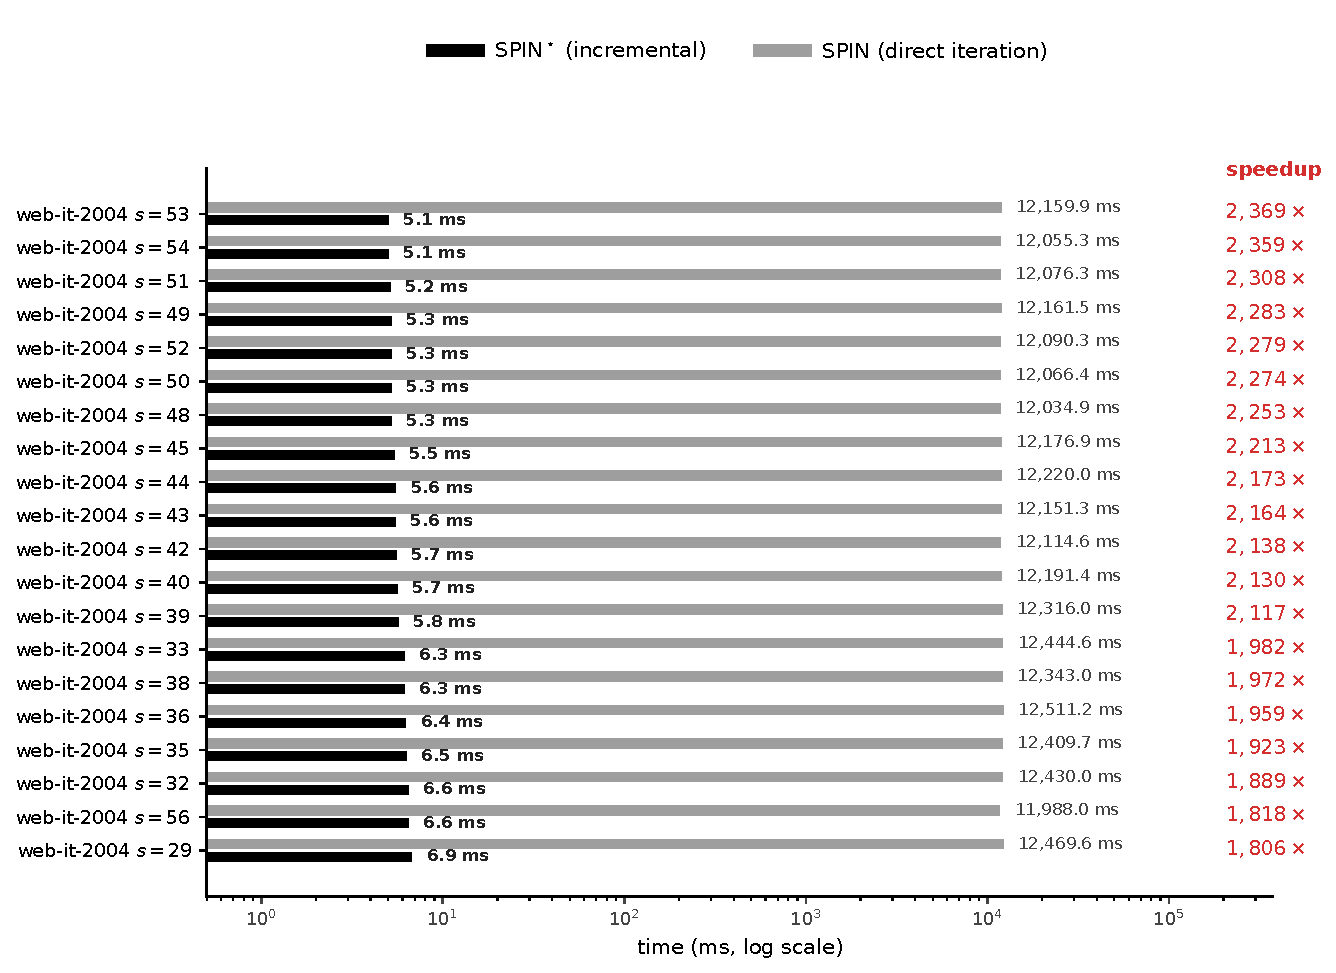
\includegraphics[width=\linewidth]{figures/fig_spin_vs_spinstar.pdf}
\caption{Per-cell wall-clock time of \spinStar{} (incremental) versus \spin{} (direct iteration), top \(20\) of the matched \((graph,s)\) cells sorted by speedup.
%
Both algorithms compute the same \((1,s)\)-core values; \spinStar{} avoids redundant full-graph passes by only revisiting vertices whose path counters changed.}
\Description{Paired horizontal bars per (graph, s) cell comparing SPIN and SPIN* wall-clock time on a log axis.}
\label{fig:spin-vs-spinstar}
\end{figure*}

\spin{}'s memory profile, with the dual-CSR data structure shared with \spinStar{}, is essentially identical to \spinStar{}'s on every paired cell: the geometric-mean RSS ratio (\spin{}\(/\)\spinStar{}) is \(0.97\) over the \(291\) matched cells, and \spin{} is slightly smaller than \spinStar{} on \(83.8\%\) of them.
%
The reason is structural: \spinStar{}'s extra state beyond the shared CPI consists of a per-path counter cache (\(\sim 13\) bytes per leaf) and a peel-order bucket queue (\(\sim 17\) bytes per vertex), which \spin{} does not maintain because it scans every vertex each round.
%
The sub-percent memory advantage of \spin{} is therefore the price \spinStar{} pays to avoid repeated full-graph passes; the trade is the textbook ``space for time'' choice, with the time term dominating by orders of magnitude.

For reference, Table~\ref{tab:localh} lists representative single-threaded \spin{} runs alongside the corresponding \spinStar{} times.

\begin{table}[t]
\centering
\caption{Representative \spin{} runs.
%
\spinStar{} time is end-to-end wall-clock time on the same \((graph,s)\) cell.}
\label{tab:localh}
\tiny
\setlength{\tabcolsep}{2pt}
\begin{tabular}{llrrrrr}
\toprule
Graph & \(s\) & \spin{} & SPIN (s) & \spinStar{} (ms) & ratio & RSS (GB) \\
\midrule
\texttt{com-amazon} & 8 & OK & \(0.0\) & \(2.6\) & \(1\times\) & \(0.1\) \\
\texttt{com-dblp} & 10 & OK & \(0.1\) & \(4.6\) & \(12\times\) & \(0.1\) \\
\texttt{com-youtube} & 5 & OK & \(11.4\) & \(144.5\) & \(79\times\) & \(0.4\) \\
\texttt{soc-pokec} & 5 & OK & \(55.2\) & \(2138.6\) & \(26\times\) & \(1.2\) \\
\texttt{wiki-Talk} & 5 & OK & \(672.9\) & \(2528.1\) & \(266\times\) & \(7.0\) \\
\texttt{web-Google} & 8 & OK & \(1.1\) & \(137.4\) & \(8\times\) & \(0.3\) \\
\texttt{web-Stanford} & 10 & OK & \(2.7\) & \(51.7\) & \(53\times\) & \(0.1\) \\
\bottomrule
\end{tabular}
\end{table}

The result is not a failure of the fixed-point view.
%
It explains why the paper needs both algorithms.
%
\spin{} gives the direct semantic formulation.
%
\spinStar{} computes the same fixed point by processing only the vertices whose witness counters changed.

\stitle{RQ5: dense synthetic stress.}
The benchmark graphs are sparse.
%
The stress test follows the dense synthetic protocol used in prior nucleus-decomposition studies~\cite{nucleusSariyuceTODS,NuclearCD}.
%
It generates \(1000\)-vertex graphs by incremental clique injection and sweeps \(12\) densities from \(0.01\) to \(0.60\) for \(s\in\{5,7,9,11\}\).
%
Both methods grow quickly as density and \(s\) increase.
%
Where both implementations finish, \spinStar{} remains below \cbnd{} in time and memory.

\begin{figure}[t]
\centering
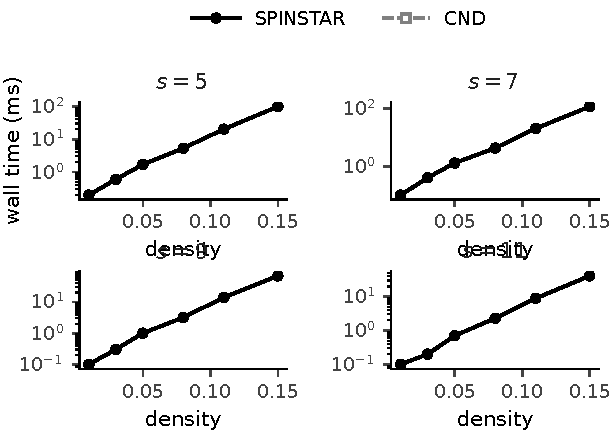
\includegraphics[width=\linewidth]{figures/fig_stress_time.pdf}
\caption{Runtime stress test on synthetic clique-injection graphs with \(|V|=1000\).
%
Solid blue is \spinStar{}, and dashed red is \cbnd{}.
%
Runtime grows rapidly as density and \(s\) increase.}
\Description{Runtime plots for synthetic dense graphs across several clique sizes and densities.}
\label{fig:stress-time}
\end{figure}

\begin{figure}[t]
\centering
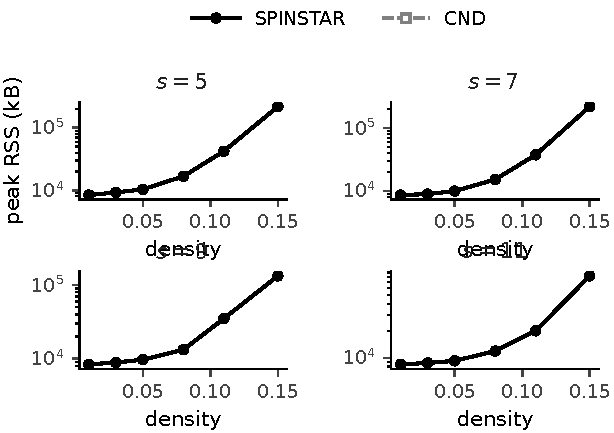
\includegraphics[width=\linewidth]{figures/fig_stress_mem.pdf}
\caption{Peak resident-set memory under the same stress-test protocol as Figure~\ref{fig:stress-time}.
%
The memory gap shows when mutable residual state amplifies dense-clique growth.}
\Description{Peak-memory plots for synthetic dense graphs across several clique sizes and densities.}
\label{fig:stress-mem}
\end{figure}

\stitle{Takeaway.}
The experiments support the paper's dependency chain.
%
\spinStar{} is faster and uses less peak memory than \cbnd{} on the \(307\) matched benchmark cells.
%
The phase breakdown shows that construction becomes a major remaining cost after peeling becomes counter-only.
%
\paraBuild{} addresses that shifted bottleneck by parallelizing static construction.
%
\spin{} confirms why the direct fixed-point view is useful for semantics but unsuitable as the practical solver.
